% !TEX root = /home/frank/School/thesis_text/thesis.tex



\chapter{Platform Overview}

\section{Zynq-7000}

The Zynq-7000 System on Chip combines a dual core ARM Cortex-A9 with Xilinx programmable logic in a single device. This combination of a CPU and an FPGA on the same device is not a new phenomenon, with examples of previous generations being the PowerPC based Xilinx Virtex-II Pro and some models of the Virtex 4 and Virtex 5 series FPGA's. A notable differences between these generations is the shift from PowerPC based architectures to ARM based architectures. Also, a notable shift in emphasis from HDL centered design to a more high-level abstraction centric view with an emphasis on high level languages can be seen. 
	

	\subsection{Processing System}
	The Zynq-7000 series SoC is split into two parts: The processing system (PS) and the programmable logic (PL). The Processing system contains an Application Processor Unit (APU), memory interfaces and I/O peripherals. 
	
		\paragraph{APU}
		The APU is a Dual ARM Cortex-A9 CPU which implements version 7 of the ARM ISA  as well as Thumb and Jazelle instruction sets. Each core has a NEON Media Processing Engine supporting SIMD vector and scalar single-precision floating-point and integer computation and scalar double-precision floating-point computation. Each core has 32 KB instruction and 32 KB data caches and there is 512 KB shared L2 cache and 256 KB of on-chip SRAM memory. The APU also has a snoop control unit to maintain L1 and L2 coherency. This snoop control unit also controls the Accelerator Coherency Port, a 64-bit AXI slave port connected to the programmable logic. The PL acts as the master and the PS as slave. This allows direct communication between the PS and the PL through the L2 caches or on chip memory with guaranteed coherency. The APU also has an on-board 8-channel DMA controller with 4-channels reserved for PS to/from memory and 4 for PL to/from memory transfers. The Processing system also contains an interrupt controller.

		\paragraph{Memory Controller}
		The Memory controller supports a number of memory technologies. The system has a DDR controller which supports DDR2 and DDR3 memory, a Quad-SPI controller which converts normal memory read operations to SPI and vice versa, and a Static Memory Controller which supports NAND and SRAM/NOR type memory.

		\paragraph{I/O Peripherals}
		The Processing system contains quite a lot of industry standard I/O peripherals for external data communication.
			\begin{multicols}{2}
				\begin{itemize}
					\item GPIO
					\item 2 Gigabit Ethernet Controllers
					\item 2 USB controllers
					\item 2 SD/SDIO controllers
					\item 2 SPI controllers
					\item 2 CAN controllers
					\item 2 UART controllers
					\item 2 I$^{2}$C controllers
				\end{itemize}
			\end{multicols}

		These peripherals are connected to multiplexed I/O buffers which enable to externalize these signals to up to 54 pins. If there is a need for more I/O pins the signals can be routed into the PL through the extended MIO, where they can be routed directly to package pins or peripherals in the PL.

	\subsection{Programmable Logic}
	The programmable logic provides the same functionality that can be expected from a Xilinx FPGA. The PL in 7z010 and 7z020 Zynq SoCs is based on Artix-7 FPGAs whereas the PL in 7z030, 7z045 and 7z100 SoCs is based on Kintex-7 FPGA logic. This PL can be coupled through a couple of different interconnects, with varying degrees of interconnectedness between the PL and the PS. Of note here is that the PS has to be booted first and the PL logic has to be configured from the PL at boot or at a later time. This is another example of the shift to a more software centered view. The system has all the features one can expect from an FPGA: configurable logic blocks with look-up tables, a number of 36 KB block RAMs, DSP348E slices and configurable IO. The PL side also contains an Analog to Digital converter, and in the larger varieties of the Zynq SoC an integrated PCI Express block.

\begin{figure}[H]
\centering
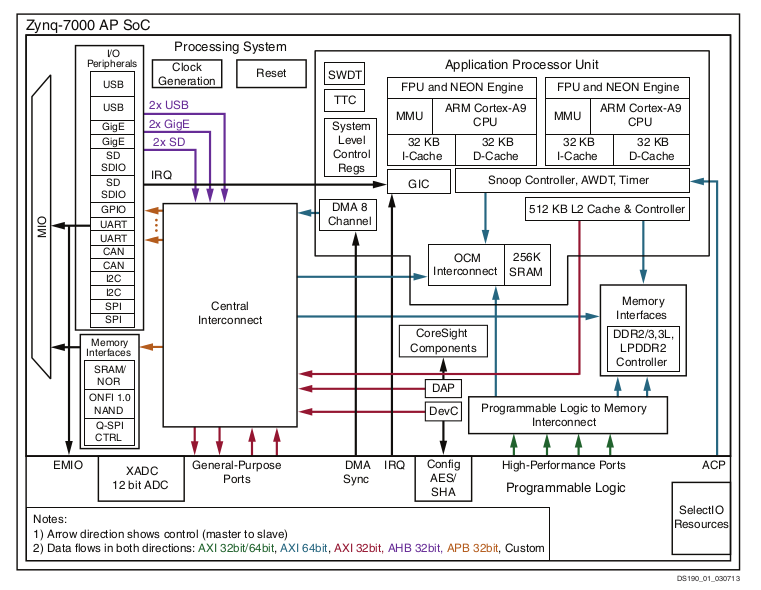
\includegraphics[scale=0.5]{/home/frank/School/thesis_text/images/zynq_block_diagram.png}
\caption{Zynq -7000 SoC overview \cite{anon._zynq-7000_2013}}
\label{img:zynq_overview}
\end{figure}

	\subsection{Interconnect}
	The interconnect system is located in the PS but because of it's influence on performance it warrants its own section. The interconnect system is comprised of a number of switches to connect the different parts of the system using the AXI point-to-point protocol. The AXI protocol is part of the ARM Advanced Microcontroller Bus Architecture version 3.0. These AXI interconnects are the primary means of communication between the PS and the PL. There are a number of different interface ports between the PS and the PL:

		\begin{description}
			\item[AXI\_HP] There are four AXI\_HP interfaces, connecting PL masters with high bandwidth datapaths to the DDR and OCM memories. Each interface is buffered with 2 FIFOs and is configurable to be 32 or 64 bits wide.
			\item[AXI\_GP] The four general purpose AXI\_GP ports are divided into 2 master ports and 2 slave ports. These ports don't have FIFO buffering which makes them less suitable for high performance use. 
			\item[AXI\_ACP] The Accelerator coherency port is a 64-bit AXI slave interface that directly connects the PL to the APU caches. This is done through the snoop control unit and can enforce coherency if requested. 
		\end{description}

	The actual interconnection is implemented through a number of switches. Amongst these are the snoop control unit, the L2 cache controller and a couple of ARM NIC-301 based interconnect switches.

		\begin{description}
			\item[Snoop Control Unit] Although the SCU is in essence not a switch, its behavior in regards to the transfer of data from its AXI slave ports to its AXI master ports makes it function as a switch.
			\item[Central Interconnect] The central interconnect is the core of the interconnect network in the Zynq SoC.\
			\item[Master Interconnect] The master interconnect connects the Master switches the traffic from the AXI\_GP ports as well as traffic coming from the device configuration core and the debug access port.
			\item[Slave Interconnect] The slave interconnect switches traffic coming from the central interconnect to AXI\_GP, I/O peripherals, APB connections, etc.
			\item[Memory Interconnect] The memory interconnect switches high speed traffic coming from the AXI\_HP ports to DDR and on-chip RAM.
			\item[OCM Interconnect] The on-chip memory connect switches the traffic from the central interconnect and the memory interconnect.
		\end{description}

		A diagram of how these interconnects are organized can be found in figure \ref{img:zynq_intereconnect}

\begin{figure}[H]
\centering
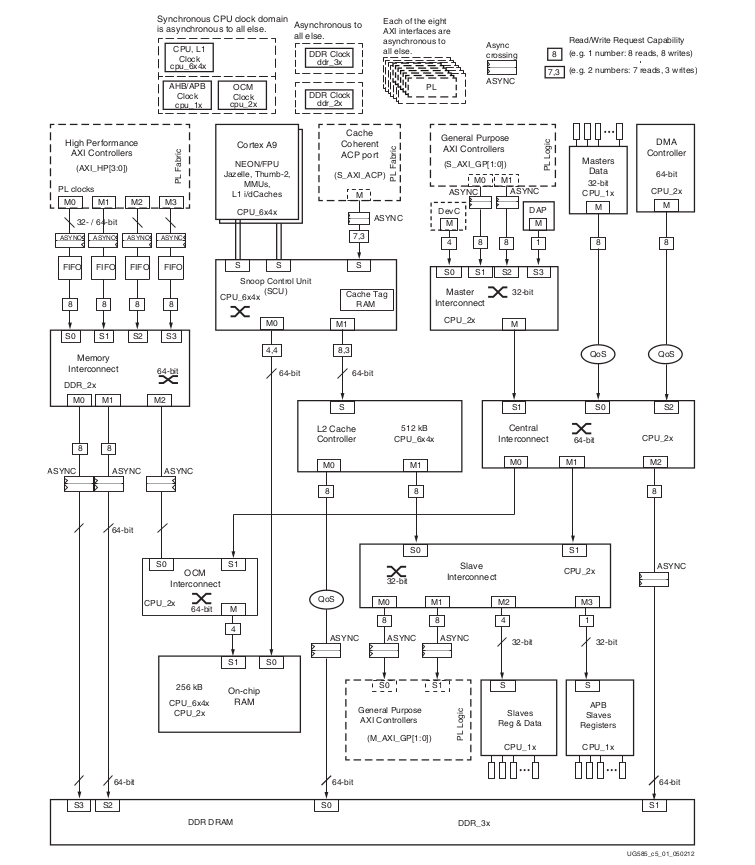
\includegraphics[scale=0.55]{./images/interconnect_block_diagram.png}
\caption{Zynq Interconnect System Block Diagram \cite{anon._zynq-7000_2013}}
\label{img:zynq_intereconnect}
\end{figure}

\newpage

\section{Toolchain}
Because of the heterogeneous nature of the Zynq Soc there are a number of tools necessary to implement a design. In this section the tools used for this thesis are discussed.

\paragraph{PlanAhead} PlanAhead is the main interface for the hardware side of a project. It allows a designer to bring together VHDL or Verilog code, IP-cores, embedded designs from Xilinx Platform studio and DSP designs from System generator. It also integrates with ISE Simulator to allow the functional verification of HDL code and IP. PlanAhead also allows the insertion of Chipscope cores to debug RTL designs.

\paragraph{Xilinx Platform Studio (XPS)} Xilinx platform studio is a graphical tool that allows a designer to build embedded processor systems including IP-cores. The connections between peripherals in the PL and the PS are made using this application.

\paragraph{Vivado HLS} Vivado HLS is a high-level synthesis tool that converts C, C++ and SystemC to synthesizable hardware. It can export this hardware into a number of formats, among which the PCore format for XPS. More on Vivado HLS can be found in section \ref{sec:vivado_HLS}

\paragraph{Xilinx SDK} Xilinx' Software Development Kit is an eclipse based integrated development environment targeting the ARM core in Zynq or the Microblaze softcore processor. It includes a complete GNU based compiler toolchain in the form of the Mentor Sourcery Codebench Lite - Xilinx edition, which also incorporates debugging and profiling tools. The SDK also has plug-ins which make it aware of the peripherals placed in the PL and drivers for Xilinx supplied IP-cores.

The necessary steps for developing a design for the Zynq SoC are as follows:

\begin{enumerate}
	\item Start the project in PlanAhead, specify the parameters of the hardware you're developing for and create a new embedded design
	\item Independent of the PlanAhead project, implement the algorithm using Vivado HLS so it satisfies all design constraints. Export the implementation as an IP-core suitable for use in XPS.
	\item In XPS, add the Vivado HLS generated IP core to the system along with other IP-cores. Make all the necessary interconnections.
	\item Add the necessary floor-planning constraints in PlanAhead. Synthesize the system, perform the implementation step on the system and generate a bitstream. Correct any errors that show up during these steps until the system is error-free.
	\item Export the system to SDK. Develop the embedded software in the IDE using the available drivers. Create a boot image combining the software and the hardware and launch the application on the hardware.
\end{enumerate}
These steps are visually represented in figure \ref{img:toolchain_diagram}

\begin{figure}[H]
\centering
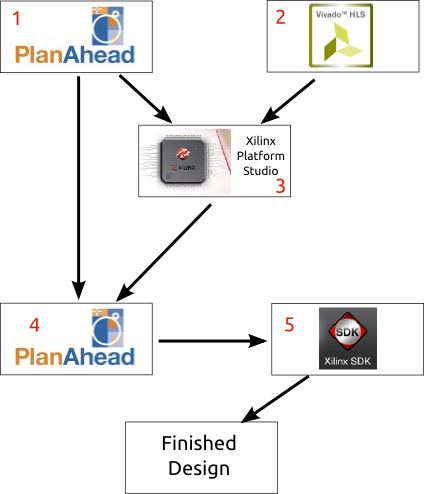
\includegraphics[scale=0.7]{./images/toolchain_diagram/toolchain_diagram.png}
\caption{Diagram of the Zynq toolchain}
\label{img:toolchain_diagram}
\end{figure}

Xilinx provides an alternative toolchain in its Vivado Design Suite. It supports the Zynq-7000 series since the release of version 2013.3 in October 2013. This software combines the functions of PlanAhead and XPS into one application. For new designs using 7-series and Zynq devices Xilinx recommends using Vivado Toolchain, With the old ISE toolchain still being available for backward compatibility reasons.\cite{isereleasenotes}.


\section{Base Targeted Reference Design 14.5}
Zynq is a powerful but complex architecture requiring a designer with a diverse skill set. Building a real-time video processing system from scratch would involve connecting multiple IP-cores to each other and to the PS, as well as writing efficient applications that use the implemented hardware. Because this falls beyond the scope of this thesis an existing design, Base Targeted reference Design version 14.5, was selected to do a performance analysis on.

\subsection{Hardware}
The hardware side can be split into 3 stages:\\ 

The first stage starts with the \emph{fmc\_imageon\_hdmi\_in} IP-core. This core extracts the horizontal and vertical blanking signals from the YCrCb 4:2:2 input it receives from the FMC-Imageon Module. In turn this core is connected to the \emph{Video In to AXI4-Stream} IP-core. This core handles the clock boundary between the video clock domain and the AXI4-Stream clock domain. The preservation of timing information is guaranteed by a Video Timing Core. The AXI4-stream is routed into a \emph{Test Pattern Generator} IP-core which can generate a test-pattern or act as a pass-through for the video signal, depending on the configuration. The data coming from the TPG is fed into a \emph{Chroma Resampler} IP-core which converts the YCrCb 4:2:2 formatted signal into a YCrCb 4:4:4 signal. HDMI uses the chroma subsampling to reduce the amount of data that needs to be transmitted. This can be done because the human eye is not as sensitive for the Chroma components as it is for the Luminance component. The upsampling is necessary for the following step, which is the colorspace conversion performed by the \emph{YCrCb to RGB Color-Space Converter} IP-core, which converts the YCrCb signal to RGB video as this is the format required by the following steps in the video processing pipeline. The video signal gets routed into a \emph{Video DMA}controller which writes the data to memory using an \emph{AXI Interconnect} IP-core connected to the PS' S\_AXI\_HP0 port.\\
The second stage has a second \emph{AXI Interconnect} IP-core connected to the PS' S\_AXI\_HP2 port. A \emph{Video DMA} controller reads data from memory through this interconnect and converts the date from the AXI memory mapped format to an AXI stream format. This gets sent to the Vivado HLS generated Sobel core. This core sends the data back to the Video DMA controller which writes it back to memory through the AXI Interconnect.
The Third and last stage consists of the Xylon logiCVC-ML which is connected to the first AXI Interconnect. This is a video display controller which reads the data from the video memory and converts it into a format suitable for output. It also generates the control signals for the output.\\
The IP-cores that use AXI-Lite for their configuration are also connected to a third AXI Interconnect IP-core. This IP-core is connected to the M\_AXI\_GP0. Through this connection the PS is able to control the functioning of the video processing pipeline. Finally there is an AXI Performance Monitor IP-core also connected to this third interconnect. The Performance monitor monitors the throughput on the S\_AXI\_HP0 and S\_AXI\_HP2 ports. 


\subsection{Software}
On the software side the TRD uses three major components:
\begin{itemize}
	\item Bootloader
	\item Xilinx Linux Kernel
	\item Application
\end{itemize}

\subsubsection{Bootloader} The TRD uses the SD card as the boot device. The bootloader is stored in the BOOT.BIN file and performs a number of functions. The system uses a two-stage bootloader. On boot the first stage bootloader gets executed. This performs the necessary initializations that enable the system to load the bitstream into the PL and execute the U-Boot bootloader. The bitstream is also contained in the BOOT.BIN file and is loaded into the PL after the initialization has finished. After the FSBL has finished it executes the second stage, the U-Boot bootloader which loads the kernel image into the DDR memory.

\subsubsection{Linux Kernel}
The TRD uses a Linux kernel that is based on the mainline Linux kernel but maintained by Xilinx. This kernel incorporates many patches not found in the mainline kernel. These patches provide support for Xilinx specific features. Supported devices include the Xylon logiCVC-ML which gets abstracted to a generic frame buffer drive, Xilinx VDMA controllers which controls the transfers to and from the DDR memory, PS-GPIO giving access to GPIO pins to the operating system, and the ADV7511 HDMI transmitter gets a Video4Linux v2 Driver. Some IP cores have limited functionality and don't warrant a complete Kernel Driver being written to support the driver. In this case the developer can use the \emph{Userspace IO} framework present in the Linux kernel.\\
The userspace IO (or UIO) is a framework present in the Linux kernel that allows a developer to write a minimal kernel driver for a piece of hardware and perform most of the necessary functions from userspace. This system reduces the complexity of driver development and reduces the risk for bugs in a kernel module. UIO is a good fit for a device if it has one or more of following properties:
\begin{itemize}
	\item The device has memory that can be mapped onto virtual memory and can be completely controlled using this memory.
	\item The device generates interrupts.
	\item The device doesn't fit in one of the standard kernel subsystems.
\end{itemize}

These UIO device drivers are made available to the user through the device node and the Sysfs, which is a virtual file system that exports information on devices and their drivers. The device file typically has the form /dev/UIOX with X being a number starting on 0. This file represents the memory of the system and can be opened using the MMAP() system call. Interrupts are handled by performing a blocking read on the device file. When the read returns an interrupt has happened. The return value is an integer which contains the number of interrupts that have occurred. By comparing this value to the previous value the user can check whether any interrupts were missed. Vivado HLS generates the UIO driver, leaving only the development of a kernel module to be done by the developer.

\subsubsection{Application}
There are 2 versions of the application available: a version with a Qt based GUI and a commandline based application. The application lets the user select one of two video sources, the TPG or the HDMI input, and apply 2 implementations of the Sobel filter on these inputs. One implementation is done in software and runs on ARM processor, the other one is a Vivado HLS generated core. The Qt application also has a readout of the system throughput.


\subsection{Sobel Operator}

The described system performs edge detection using the Sobel operator on the video data. The Sobel operator computes an approximation of the gradient. The computation is done by convolving the image with 2 $3 \times 3$ kernels.

\begin{equation}
G_{x} = 
\begin{bmatrix}
+1 & 0 & -1 \\
+2 & 0 & -2 \\
+1 & 0 & -1
\end{bmatrix}
\hspace{20mm}
G_{y} = 
\begin{bmatrix}
+1 & +2 & +1 \\
0 & 0 & 0 \\
-1 & -2 & -1 \\
\end{bmatrix}
\end{equation}

The combination of these operators give an approximation of the gradient in both the x and the y direction. The sum of the absolute values of these two approximations gives the edge weight. It shows whether a location is close to an abrupt change in intensity in an image, an edge. By thresholding the edges can be separated from the rest of the image. The Vivado HLS code implementing this is given in listing \ref{lst:sobeloperator}. The Sobel operator falls under dwarf number 6: structured grid which puts it in the cross section of the CPU, GPGPU and FPGA categories. The sobel operator is thus a good fit for the Zynq platform.

\begin{lstlisting}[caption=Sobel operator implementation, captionpos=b, label=lst:sobeloperator]
  for(i=0; i < 3; i++){
    for(j = 0; j < 3; j++){

      // X direction gradient
      x_weight = x_weight + (window->getval(i,j) * x_op[i][j]);
      
      // Y direction gradient
      y_weight = y_weight + (window->getval(i,j) * y_op[i][j]);
    }
  }
  
  edge_weight = ABS(x_weight) + ABS(y_weight);

  if (edge_weight < 255)
  edge_val = (255-(unsigned char)(edge_weight));
  else
  edge_val = 0;

  //Edge thresholding
  if(edge_val > high_thesh)
    edge_val = 255;
  else if(edge_val < low_thresh)
    edge_val = 0;
\end{lstlisting}

